%!TEX root = ./ai-jst.tex
%-------------------------------------------------------------------------------
%                            BAB II
%               TINJAUAN PUSTAKA DAN DASAR TEORI
%-------------------------------------------------------------------------------

\chapter{KAJIAN LITERATUR}                

\section{Tinjauan Pustaka}
 Jaringan syaraf tiruan (JST) merupakan salah satu representasi buatan dari otak manusia yang selalu mencoba mensimulasikan proses pembelajaran otak manusia tersebut. Jaringan Syaraf Tiruan tercipta sebagai suatu generalisasi model matematis dari pemahaman manusia (\emph{human cognition}) yang didasarkan atas asumsi berikut:
 \begin{enumerate}
 	\item Pemrosesan informasi terjadi pada elemen sederhana yang disebut neuron.
 	\item Isyarat mengalir di antara sel syaraf (neuron) melalui suatu sambungan penghubung.
 	\item Setiap sambungan penghubung memiliki bobot yang bersesuaian.
 	\item Setiap sambungan penghubung memiliki bobot yang bersesuaian.
 	\item Setiap sel syaraf akan merupakan fungsi aktivasi terhadap isyarat hasil penjumlahan
 	berbobot yang masuk kepadanya untuk menentukan isyarat keluarannya \cite{ZeksonArizonaMatondang}
 \end{enumerate}

\section{Landasan Teori}
 \subsection{Jaringan Syaraf Tiruan \emph{Artificial Neural Network}}
 Jaringan Syaraf Tiruan atau \emph{Artificial Neural Network} merupakan sistem pemrosesan informasi tertentu yang memiliki kinerja secara umum menyerupai jaringan syaraf biologis. JST merupakan model matematika yang digeneralisasikan dari jaringan syaraf biologi, berdasarkan dari asumsi diatas maka dapat kita artikan:
 \begin{enumerate}
 	\item Pemrosesan infromasi terjadi pada elemen sederhana yang dipanggil \emph{neuron}
 	\item Sinyal akan diteruskan diantara \emph{neuron-neuron} melalui jaringan penghubung.
 	\item Masing-masing penghubung mempunyai \emph{weight} nya sendiri-sendiri, dimana pada setiap \emph{weight} akan di kalkulasi pada tiap penerusan sinyal.
 	\item Masing-masing \emph{neuron} akan menjalankan fungsi aktivasi (umumnya pada model-model \emph{non-linear}) terhadap sinyal yang diteruskan (jumlah dari \emph{weight} sinyal yang masuk) untuk menentukan nilai sebenarnya dari sinyal.
 \end{enumerate}
Sebuah model JST ditandai dengan (1) pola dari koneksi atau penghubung antara \emph{neuron-neuron}nya (biasanya dipanggil arsitektur), (2) metode yang digunakan untuk menentukan \emph{weight} atau bobot (dinamakan \emph{training} atau \emph{learning, algorithm}) dan (3) fungsi aktivasinya \cite{fausett1994fundamentals}

\subsection{Arsitektur Jaringan Syaraf Tiruan}
Jaringan syaraf tiruan memiliki beberapa arsitektur jaringan yang sering digunakan dalam berbagai aplikasi. Arsitektur jaringan syaraf tiruan tersebut antara lain:
\begin{enumerate}
	\item Jaringan Tunggal (\emph{sigle layer network}) \par 
	Pada jaringan ini sekumpulan \emph{nerual} yang menjadi \emph{input} terhubung langsung dengan \emph{output}. Sinyal mengalir searah dari dari \emph{neuron input} ke \emph{neuron output}.
	 \begin{figure}[H]
		\centering
		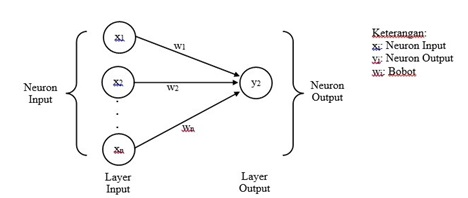
\includegraphics{gambar/net-1}
		\caption{\emph{Single layer neural network}\protect\footnotemark}
		\label{JST-1}
	\end{figure}
	\footnotetext{sumber: https://socs.binus.ac.id/files/2017/03/lili-1.jpg}
	\item  Jaringan syaraf jamak (\emph{multilayer network}) \par 
	Jaringan dengan lapisan jamak memiliki ciri khas tertentu yaitu memiliki 3 jenis
	\emph{layer} yakni \emph{input}, \emph{output layer}, dan \emph{hidden layer}. Jaringan dengan banyak
	lapisan ini dapat menyelesaikan permasalahan yang kompleks dibandingkan jaringan
	dengan lapisan tunggal. Namun proses pelatihan sering membutuhkan waktu yang
	cenderung lama. Contoh algoritma jaringan syaraf tiruan yang menggunakan metode
	ini yaitu : Madaline, backpropagation, neocognitron.
	\begin{figure}[H]
		\centering
		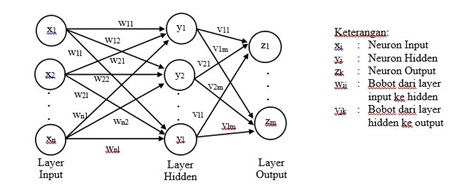
\includegraphics{gambar/net-2}
		\caption{\emph{Multi layer neural network}\protect\footnotemark}
		\label{JST-2}
	\end{figure}
	\footnotetext{sumber: https://socs.binus.ac.id/files/2017/03/lili-3.jpg}
\end{enumerate}

\subsection{Metode Propagasi Balik (\emph{Backpropagation Algorithm})}
Sebenarnya ada banyak metode yang bisa digunakan dalam melakukan \emph{training} atau \emph{learning algorithm} didalam sebuah model jaringan syaraf tiruan, namun pada model klarifikasi dan penetuan tugas akhir mahasiswa ini kami mengunakan metode \emph{backpropagation}. \par 
\emph{Backpropagation} merupakan sebuah metode yang melalui tiga fase, antara lain:
\begin{enumerate}
	\item Propagasi Maju (\emph{FeedForward Propagation}) \par 
	Selama propagasi maju, sinyal masukan (= x\textsubscript{i}) dipropagasikan ke lapis tersembunyi menggunakan fungsiaktivasi yang ditentukan. Keluaran darisetiap unit lapis tersembunyi (= z\textsubscript{j}) tersebut selanjutnya dipropagasikan majulagi ke lapis tersembunyi di atasnya menggunakan fungsi aktivasi yang ditentukan. Demikian seterusnya hingga menghasilkan keluaran jaringan (= y\textsubscript{k}). \par 
	Berikutnya, keluaran jaringan (= y\textsubscript{k}) dibandingkan dengan target yang harus
	dicapai (= t\textsubscript{k}). Selisih t\textsubscript{k} - y\textsubscript{k} adalah kesalahan yang terjadi. Jika kesalahan ini lebih kecil dari batas toleransi yang ditentukan, maka iterasi dihentikan. Akan tetapi apabila kesalahan masih lebih besar dari batas toleransinya, maka bobot setiap garis dalam jaringan akan dimodifikasikan untuk mengurangi kesalahan yang terjadi.
	
	\item Propagasi Mundur (\emph{Backpropagation}) \par 
	Berdasarkan kesalahan t\textsubscript{k} - y\textsubscript{k}, dihitung faktor b\textsubscript{k} (k=1, 2, …, m) yang dipakai	untuk mendistribusikan kesalahan di unit y\textsubscript{k} ke semua unit tersembunyi yang terhubung langsung dengan y\textsubscript{k}. b\textsubscript{k} juga dipakai untuk mengubah bobot garis yang menghubungkan langsung dengan unit keluaran. Dengan cara yang sama, dihitung di setiap unit di lapis tersembunyi sebagai dasar perubahan bobot semua garis yang berasal dari unit tersembunyi di lapis di bawahnya. Demikian seterusnya hingga faktor b di unit tersembunyi yang berhubungan langsung dengan unit masukan dihitung. 
	
	\item Perubahan Bobot (\emph{Weight Update}) \par 
	Setelah semua faktor b dihitung, bobot semua garis dimodifikasi bersamaan.
	Perubahan bobot suatu garis didasarkan atas faktor b neuron di lapisatasnya. Sebagai
	contoh, perubahan bobot garis yang menuju ke lapis keluaran didasarkan atas dasar b\textsubscript{k}
	yang ada di unit keluaran. Ketiga fase tersebut diulang terus hingga kondisi penghentian
	dipenuhi. Umumnya kondisi penghentian yang sering dipakai adalah jumlah iterasi atau
	kesalahan. Iterasi akan dihentikan jika jumlah iterasi yang dilakukan sudah melebihi
	jumlah maksimum literasi yang ditetapkan, atau jika kesalahan yang terjadi sudah lebih
	kecil dari batas toleransi yang diijinkan
	
\end{enumerate}

\subsection{Fungsi aktivasi (\emph{Sigmoid})}
Fungsi aktivasi sigmoid ini digunakan untuk jaringan saraf yang dilatih
dengan menggunakan metode backpropagation. Fungsi sigmoid memiliki nilai pada
range 0 sampai 1. Oleh karena itu, fungsi ini sering digunakan untuk jaringan saraf
yang membutuhkan nilai output yang terletak pada interval 0 sampai 1. Namun,
fungsi ini bisa juga digunakan oleh jaringan saraf yang nilai outputnya 0 atau 1. \par 
Fungsi sigmoid dirumuskan sebagai berikut :
\begin{center}
	$$ F(x) =  \frac{\mathrm{1} }{\mathrm{1} + e^-x }  $$ 
\end{center}

\newpage
\par 
Fungsi Step dirumuskan sebagai berikut : 
\begin{center}
	$$  𝑦′(𝑥) = 𝑓(𝑥)(1 − 𝑓(𝑥)) $$
\end{center}
\par 
Grafik dari fungsi sigmoid bisa dilihat sebagai berikut : 
\begin{figure}[H]
	\centering
	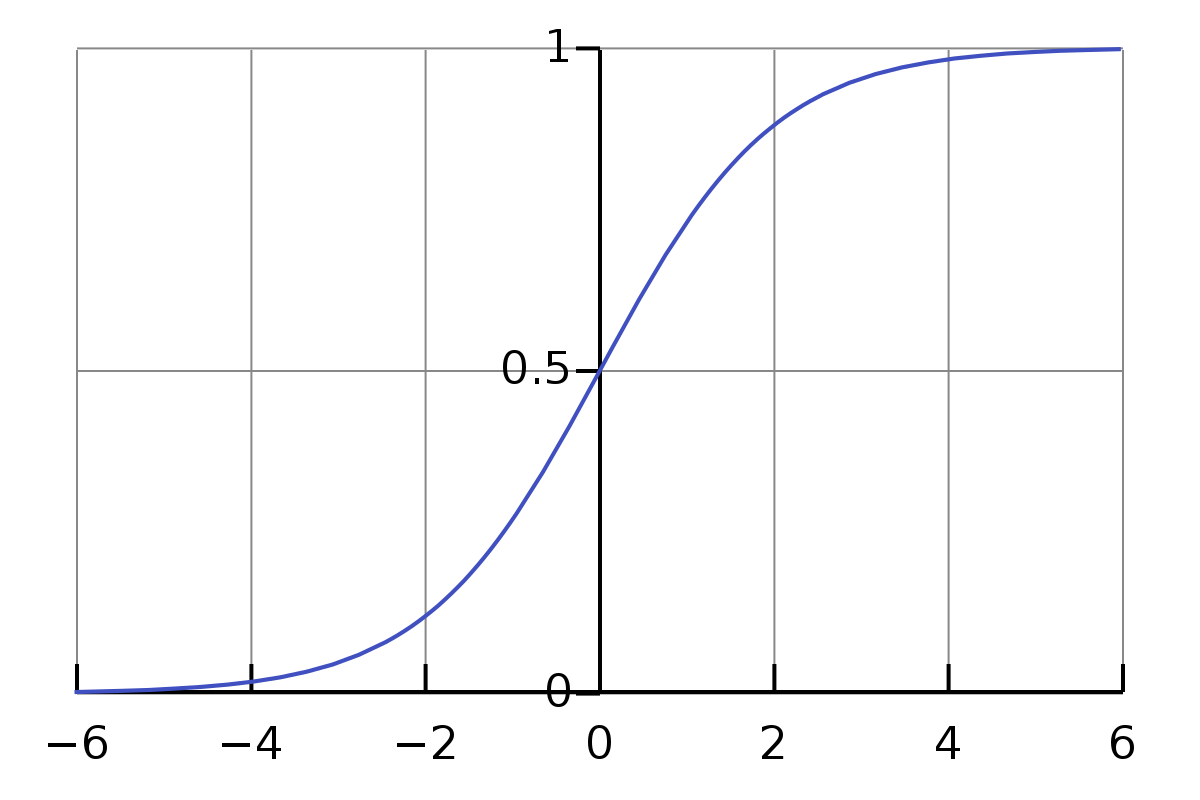
\includegraphics[width=10cm]{gambar/sigmoid}
	\caption{Grafik fungsi \emph{sigmoid}\protect\footnotemark}
	\label{JST-2}
\end{figure}
\footnotetext{sumber:https://upload.wikimedia.org/wikipedia/commons/thumb/8/88/Logistic-curve.svg/1200px-Logistic-curve.svg.png}

\par 
Fungsi sigmoid memiliki nilai maksimum = 1. Maka untuk pola yang
targetnya > 1, pola masukan dan keluaran harus terlebih dahulu ditransformasi
sehingga semua polanya memiliki range yang sama seperti fungsi sigmoid yang
dipakai. Alternatif lain adalah menggunakan fungsi aktivasi sigmoid hanya pada
layar yang bukan layar keluaran. Pada layar keluaran, fungsi aktivasi yang dipakai
adalah fungsi identitas : $ 𝑓(𝑥) = 𝑥 $.
% Baris ini digunakan untuk membantu dalam melakukan sitasi
% Karena diapit dengan comment, maka baris ini akan diabaikan
% oleh compiler LaTeX.
\begin{comment}
\bibliography{daftar-pustaka}
\end{comment}
